\chapter{THE REVERSE MAPPING PROBLEM}
\thispagestyle{plain}

\label{ReverseMapping}

The reverse-mapping problem is the problem of defining a function $f^{-1}$ that maps a system-level configuration $\mathbf y$ onto a solution space $\hat{\mathbf S}$ that represents all possible configurations that would have the system exhibit $\mathbf y$:
   \[ f^{-1}(\mathbf y) \rightarrow \hat{\mathbf S}. \]
Every configuration $\hat {\mathbf x} \in \hat {\mathbf S}$ should satisfy the constraint $f(\hat{\mathbf x}) \approx \mathbf y$, where $f$ is the forward mapping.
That is, $\hat{\mathbf S}$ contains all the points that would predict $\mathbf y$ in the forward mapping.

In this chapter, I give details of how \fw approaches the solution to this problem, in general, then delves deeper into actual implementations of the solution.
Then, I discuss evaluation criteria for implementations of reverse-mapping problem solutions.

\section{The \fw Approach}

The general approach taken by \fw for solving the reverse-mapping problem is similar to the \fw forward-mapping solution approach.
First, the different system-level properties are split into sub-problems.
Next, solution spaces for each sub-problem are constructed with a forward-mapping inversion technique.
Finally, each solution subspace is recombined to produce the space of configurations that will produce the provided system-level property.

Much like the forward-mapping solution, $\mathbf y$ is split into subspaces to simplify the problem:
\[ \mathbf y = \{y_0, y_1, \ldots, y_{|\mathbf y|}\}. \]
The solution space is split up in a similar manner:
\[ \hat{\mathbf S} = \{\hat S_0, \hat S_1, \ldots, \hat S_{|\mathbf S|}\}. \]
By performing this split, each forward mapping can be inverted independently:
\[ f^{-1}_i(y_i) \rightarrow \hat S_i. \]

Recombining the individual $\hat S_i$ into $\hat{\mathbf S}$ is not as simple as recombining individual $\hat y_i$ into $\hat{\mathbf y}$ in the forward-mapping solution.
Since each solution space represents which configurations satisfy a particular system-level requirement, the solution space $\hat{\mathbf S}$ is the intersection of all these spaces:
\[ \hat{\mathbf S} = \hat S_0 \cap \hat S_1 \cap \ldots \cap \hat S_{|\mathbf S|}.\]
All points at the intersection of these spaces should satisfy all system-level properties at once.

The nature of the solution spaces vary from approach to approach.
In the approaches used by \fw, they are represented as a collection of discrete subspaces, discrete exemplar points, sets of functions, or linear combinations.

\section{Reverse-Mapping Solver Implementations}

I have devised and evaluated a number of different approaches for solving the reverse-mapping problem in this dissertation research.
This section enumerates these approaches.

Although each the approaches are quite different, they all \textit{invert} a solution to the forward-mapping problem.
That is, they use the forward mapping to develop the reverse mapping, instead of learning the reverse mapping directly.
This has the benefit that the reverse-mapping solutions are agnostic to the regression method used to learn the forward mapping.

In general, these reverse-mapping solver approaches are building an invertible approximation of the forward mapping, since often times the regression approach used is not invertible.
I have found that inverting even the simplest approaches such as K-nearest neighbor and LOESS are either difficult to implement or computationally expensive.
By approximating a representation of the forward mapping that is invertible, solving the reverse-mapping problem becomes computationally tractable.
The process of inverting a method directly is covered in Subsection \ref{subsec:funcinvert}.
These approaches are generally not preferred over other approaches since they are dependent on the forward mapping approach used.
The other approximation approaches are applicable to more domains.

Each approach follows a different technical process, but all query the forward mapping for points instead of using the original data set.
Most approaches conform to the assumption stated in Chapter \ref{ForwardMapping}: The Forward-Mapping Problem that all the system-level properties can be analyzed independently.
Every approach has a different method for intersecting the different solution spaces to find a solution space that satisfies all system-level properties at once.

Each approach has different computational and space complexity.
The expectations for each method and the situations in which they are optimal vary from domain to domain and from query to query.

The first two approaches discussed in this section, \textit{Thresholding} and \textit{Simplical Complex Inversion}, conform to the theoretical framework outlined above.
Two other approaches are labeled as alternatives, as they do not follow the framework exactly, but perform a similar task.
In the final subsections, I discuss two special cases in which the system-level property is a binary value (i.e., the forward mapping is classification), or the forward mapping is one-to-one.
Throughout this section, I use the NetLogo Fires ABM\footnote{More on the Fires model is discussed in Section \ref{sec:Fires}} as an example.
The Fires domain is simple, but has solution spaces that are easy to visualize.
Other domains, such as Wolf Sheep Predation, have too many dimensions to make graphing feasible.
The arguments made with the aid of the Fires domain scale to larger dimensions.


\begin{figure}[ht]
\centering
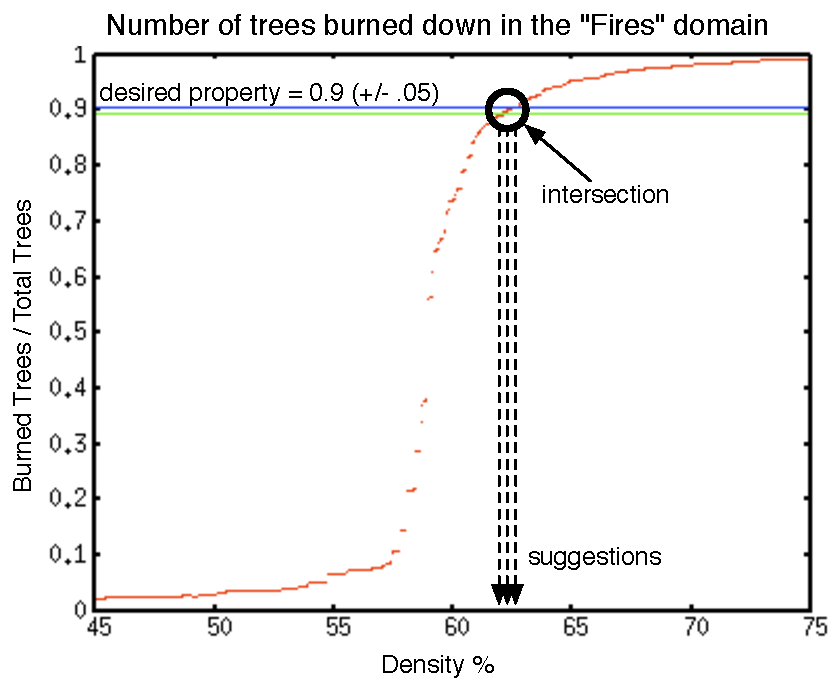
\includegraphics[scale=.66666667]{images/firesthreshold.pdf}
\caption{An illustration of the \textit{thresholding} approach to the reverse-mapping problem.}
\label{fig:firethresh}
\end{figure}

\subsection{Thresholding}

The simplest of the approaches discussed in this dissertation is dubbed the \textit{thresholding} approach.
In this approach, all points within some margin $\varepsilon$ from the system-level property $y$ are returned.
For example, all sampled points near .9 would be returned if we wanted a configuration that would yield about 90\% of the trees burned down in the Fires ABM.
Figure \ref{fig:firethresh} is an illustration of applying the thresholding approach to a data set collected for the Fires domain.
The points within this threshold are an approximation of the \textit{intersection} between the $y=.9$ plane (the horizontal lines) and the behavior space (the dots).
Configuration points that are part of this intersection are expected to produce values close to $y=.9$.
In a 600 point data set and $\varepsilon=.005$, nine points are returned that suggest configurations from 62.1 to 62.5.

This approach typically requires a large data set.
With smaller data sets, sometimes a threshold may not contain any points where there is a lot of change.
For example, no points exist between .4 and 5.5 in the 600 point data set shown in Figure \ref{fig:firethresh}.
Also, in a domain with some variance, some outliers from distant parts of the space may be included in within the threshold.
To remedy this situation, the data set can be augmented (or replaced) with a multitude of inferred points by using the forward mapping.
The data set shown in \ref{fig:firethresh} consists of interpolated points, instead of raw points (see \ref{fig:rii0} for a comparison).
The size of this data set can be made arbitrarily large given enough computation time.
Now, the threshold approach can be used and a large number of points will be returned.

There is another benefit to using inferred points over the raw data points.
The inferred points are ``smoothed" because the magnitude of the errors from neighboring points effectively cancel each other out.
These points will be even more accurate than the raw points, assuming that the forward mapping does not exhibit unseen bias.
This is because inferred points may be closer to the mean than their raw counterparts.

This approach requires O($N$) time (where $N$ is the number of points in the data set) because each point is checked to see whether it lies within the threshold.
This process can be sped up dramatically by segregating the configuration space into discrete bins.
For each bin, the minimum and maximum values for the system-level property are noted.
Now, instead of checking each point, each bin is checked to see if it could possibly contain points of the given system-level property value (i.e., the desired value is between the minimum and maximum values of the bin).
Once the candidate bins have been selected, the points in the individual bins are inspected more closely.
The same points are returned that would have been returned with the naive implementation, but without having to scan many of the points.
The pre-processing step of segregating points into bins is done offline once, and thus its computational requirement is amortized over all queries.

In comparison to the next approach discussed in this chapter, thresholding is the simplest to implement.
However, the mapping is a set of discrete points, which has limited usefulness.
Additional techniques must be applied to the solution set in order to gain any sort of high-level view.

\subsection{Simplical Complex Inversion}

Perhaps the most advanced technique \fw uses to solve the reverse mapping is \textit{Simplical Complex Inversion} (SCI).
This approach has three phases.
First, regression is used to infer the system-level property values for several ``knots" in the configuration space.
The location of these knots are used to segregate the configuration space into a number of simplexes (multi-dimensional triangles).
This segregated configuration space is referred to as a \textit{simplical complex}.
Next, the intersection between each of these simplexes and a plane representing the target system-level property is found.
That is, SCI finds the equation of the hyperplane through a simplex that satisfies the target system-level property
A curve representing the configurations that would satisfy the target system-level property is pieced together from all the intersections found.
This subsection discusses these steps in detail along with Figure \ref{fig:ISFlow}, which illustrates the SCI process.

I claim that SCI is a general approach that is applicable in all domains in which the forward-mapping problem is solved accurately.
Also, SCI provides the most useful information out of all the techniques presented in this chapter.
Instead of the discrete set of points returned by the threshold approach, SCI returns a piecewise and continuous set of hyperplanes.
These hyperplanes give a more continuous and complete view of the nature of a specific system-level property value.

\begin{figure}[ht]
\centering
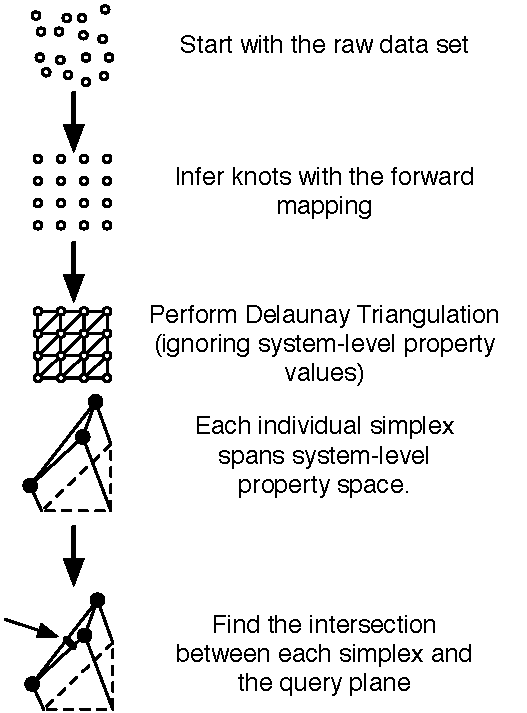
\includegraphics[scale=1]{images/ISflow.pdf}
\caption{The flow of stages in the Simplical Complex Inversion approach to the reverse-mapping problem in a two-dimensional configuration space.}
\label{fig:ISFlow}
\end{figure}


\begin{figure}[ht]
\centering
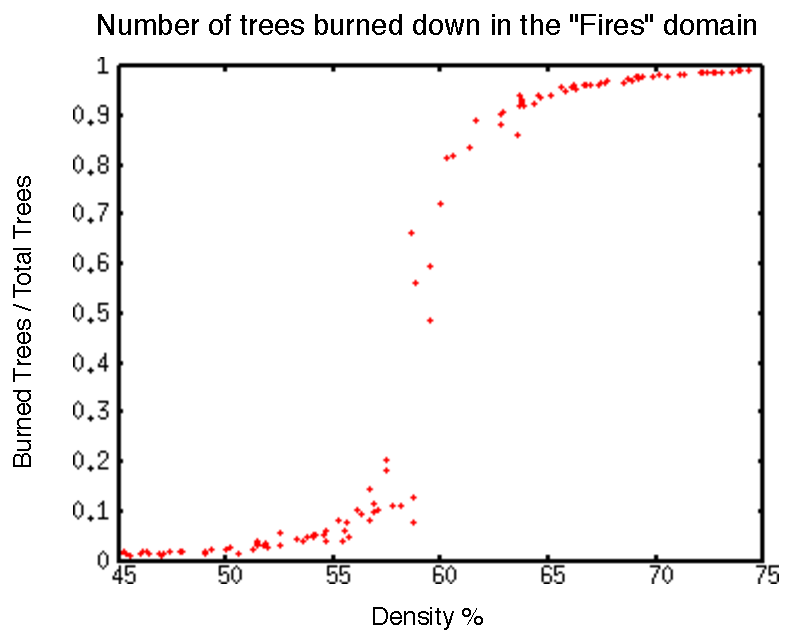
\includegraphics[scale=.66666667]{images/rii0.pdf}
\caption{The raw data set, containing 120 points, from the Fires domain.}
\label{fig:rii0}
\end{figure}

\begin{figure}[ht]
\centering
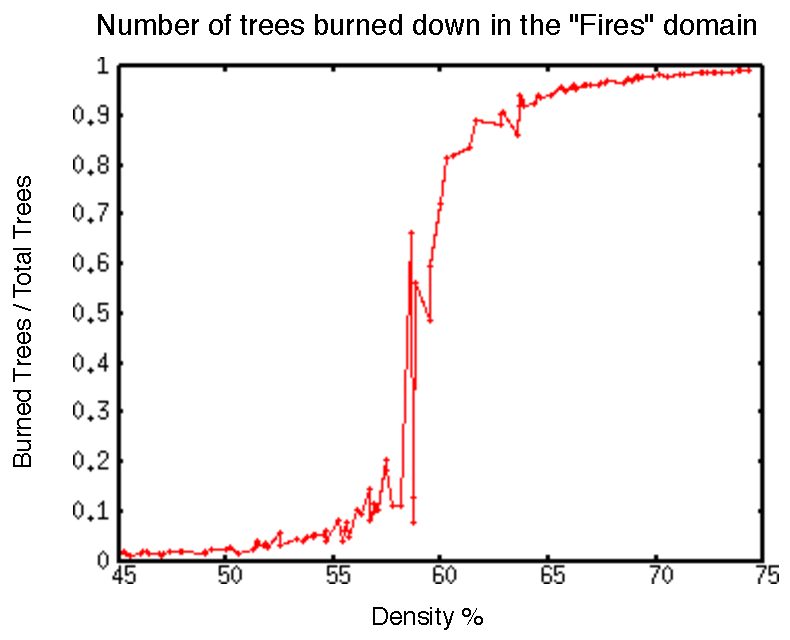
\includegraphics[scale=.66666667]{images/rii1.pdf}
\caption{Linear interpolation performed on the raw data set (see Figure \ref{fig:rii0}) from the Fires domain.}
\label{fig:rii1}
\end{figure}

\subsubsection{Segregating the Configuration Space}
The reason for using regression as the first step is the same as for using inferred points instead of the raw data set in the threshold approach.
The raw data in many ABMs will exhibit variance.
For example, raw data from the Fires ABM is shown in Figure \ref{fig:rii0}
If this data were to be used when interpolating, the curve for the behavior space would be very erratic.
This is a problem for SCI because erratic curves will result in a number of inaccurate intersections.
A linear interpolation performed on the raw Fires data to generate a behavior space curve is shown in Figure \ref{fig:rii1}.
From this figure, the curve appears very erratic and would provide poor results with SCI.


The behavior space is naturally much smoother when regression is used.
The first step is to use the forward mapping (i.e., regression) to infer knots in the space.
These knots canvas the space and provide reference points for the interpolation.
To generate these points, the forward mapping is queried by passing a configuration parameter.
An inferred system-level property value is returned.
The data knot in an $n$-dimensional\footnote{$n$ refers to the dimensionality of the configuration space for the rest of this subsection.}  configuration space is the configuration space parameter values ($x_k$) and the system-level property value ($y$):
\[(x_1, x_2, ..., x_n, y).\]

The space is then segregated into adjacent simplexes that cover the entire configuration space as a simplical complex.
These simplexes have $n + 1$ corners (e.g., triangles if $n=2$ and lines if $n=1$) and spans $(n+1)$-dimensional space.
Note that the behavior space resides in $(n+1)$-dimensional space, but the simplexes are $n$-dimensional object (e.g., a tetrahedron in four-dimensional space if $n=3$ space or a line segment in two-dimensional space if $n=1$).
The relationships between these objects' dimensionality and different dimensional configuration spaces are outlined in Table \ref{table:dims}.
For example, in the Fires ABM (1-dimensional configuration space), the space is segregated into line segments that reside in two-dimensional space.

\begin{table}[ht]
  \caption{Dimensionality of Objects for Simplex Inversion}
  \centering
  \begin{tabular}{c c c c}
    \hline \hline
    Configuration Space & Behavior Space & Simplex & Intersection \\
    Dimensionality      & Dimensionality &         &  \\
    \hline
    1 & 2 & line & point \\
    2 & 3 & triangle & line \\
    3 & 4 & tetrahedron & plane \\
    4 & 5 & pentachoron & 3D hyperplane \\
    5 & 6 & 5-simplex & 4D hyperplane \\
    $\vdots$ & $\vdots$ & $\vdots$ & $\vdots$ \\
    $n$ & $n + 1$ & $n$-simplex & ($n-1$)D hyperplane \\
    \hline
  \end{tabular}
  \label{table:dims}
\end{table}

The segregation used in SCI is a Delaunay triangulation.
If the configuration points were randomly scattered, a standard algorithm for computing the Delaunay triangulation could be used to segregate the space.
However, since SCI controls how configuration points are distributed, it can organize the points in such a way where a deterministic solution to the Delaunay triangulation can be computed implicitly.
In general, SCI will evenly space the sample points as a grid and split each hypercube into two simplexes.
The Delaunay triangulation is easy to compute with points organized in this way.
For example, in Figure \ref{fig:ISFlow}, the space is segregated into a number of adjacent triangles that satisfy the requirements for being a Delaunay triangulation.

The equations of the simplexes can be defined in terms of the hyperplane in which they reside.
The $n+1$ points define a $n$-dimensional hyperplane.
If a point is within all the facets and lies on the hyperplane, the point is on the simplex.
For example, in the Fires ABM, the two points defining a line segment reside on a more general line.
Meanwhile, the facets are defined by the points individually.
If a behavior space point lies on th line and resides between the two facet points, the point is a realistic point.
This explanation expands to two-dimensional configuration spaces, which has triangles as simplexes and line segments are facets.
If a point lies on the plane defined by the 3 points, and is within the boundaries of the line segment facets, the point is realistic.


\begin{figure}[ht]
\centering
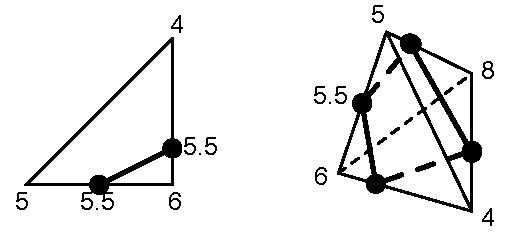
\includegraphics[scale=1]{images/simint.pdf}
\caption{A triangle from a two-dimensional configuration space (left) and a tetrahedron from a three-dimensional configuration space (right) are intersected with the plane $y=5.5$. The $y$-values for each corner are given.}
\label{fig:simint}
\end{figure}

\subsubsection{Simplex Intersection}
Recall that the final goal of this process is to find the equation of the intersection between all the simplexes and a system-level property hyperplane.
Therefore, no complicated technique needs to be performed to calculate the actual equation of the simplex or the facets.
To process to find the intersection between the system-level property hyperplane and a simplex is as follows:
\begin{enumerate}
   \item Pair off each corner with every other corner, in every possible combination. These points define the edges of the simplex.
   \item Determine which edges intersect with the hyperplane. An edge intersects with the hyperplane if the target system-level property value  is between the $y$-values for the two points that define the edge. From the intermediate-value theorem, the plane must intersect with this line segment at some point, at least once.
   \item Use linear interpolation to determine at which point on the edge line segment the intersection occurs. For example, consider the corners have $y$-values of 2 and 4 and the target system-level property value is 3---the location of the intersection is halfway between these points.
   \item After this is done for each edge, the set of all intersection points lie on the hyperplane that intersects the simplex.
\end{enumerate}
This approach totally circumvents the need for modeling the actual simplexes as equations, which can be challenging to implement.
Instead, the intersection at the edges is found by finding the intersections with the edges.
Two illustrative examples of this intersection method being used are shown in Figure \ref{fig:simint}.
In the example on the right in Figure \ref{fig:simint}, the two-dimensional plane intersects the tetrahedron in four places.
However, only three of these points are needed to define the plane because the fourth point is coplanar and thus redundant.
This illustrates the fact that not every edge has to be checked for intersection, only enough points to define the intersecting hyperplane.
Since the intersecting hyperplane is $(n-1)$D, $n$ points are needed.
This approach is very general and will work in most cases, however, when the plane intersects with either a point or an edge only, no plane can be defined because not enough non-colinear points can be found.
To circumvent this problem, SCI considers the boundaries of the simplex as not part of the simplex.
Thus, a point that intersects with only the corner or an edge will not be considered in the final piecewise intersection.


\subsubsection{Granularity}

SCI can be configured by adjusting the granularity of the knots.
SCI approximates an invertible continuous representation of the forward-mapping.
Therefore, as the granularity of SCI increases, it models the forward mapping more accurately, \textit{not} the original target domain.
Thus, the granularity should be as high as computationally acceptable.

The effect of the granularity on accuracy is dependent on the nature of the forward-mapping regression method used.
If the forward-mapping produces overfit or otherwise inaccurate predictions, the reverse-mapping produces will be inaccurate as well when it comes to suggesting behavior for the target domain.
This difficulty should be dealt with in the forward-mapping solving step, not the reverse-mapping solving step.
This is because the purpose of SCI is to model the forward-mapping, not the domain.

An empirical analysis of the relationship between granularity and accuracy is provided in Chapter \ref{Results}.
The accuracy is measured as the difference between the continuous forward-mapping function


\subsubsection{Example: Fires ABM}

Figure \ref{fig:rii} illustrates the progression of SCI from step to step when used for the Fires ABM.
First, the forward-mapping problem is solved, with whichever regression method.
Then, the knots are formed in evenly spaced intervals: in this case intervals of 1\% (see top right image in Figure \ref{fig:rii}).
The simplexes in the case of the Fires ABM are line segments, since the configuration space is one-dimensional.
Therefore, linear interpolation between the points produces these simplexes (see bottom left image in Figure \ref{fig:rii}).
This one segment is also the only edge of the simplex.

\begin{figure}[ht]
\centering
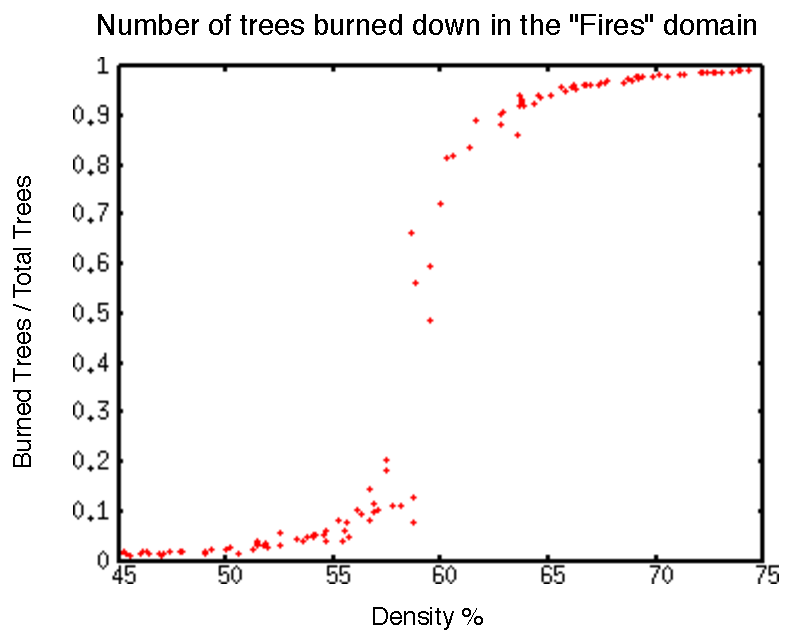
\includegraphics[scale=.5]{images/rii0.pdf}
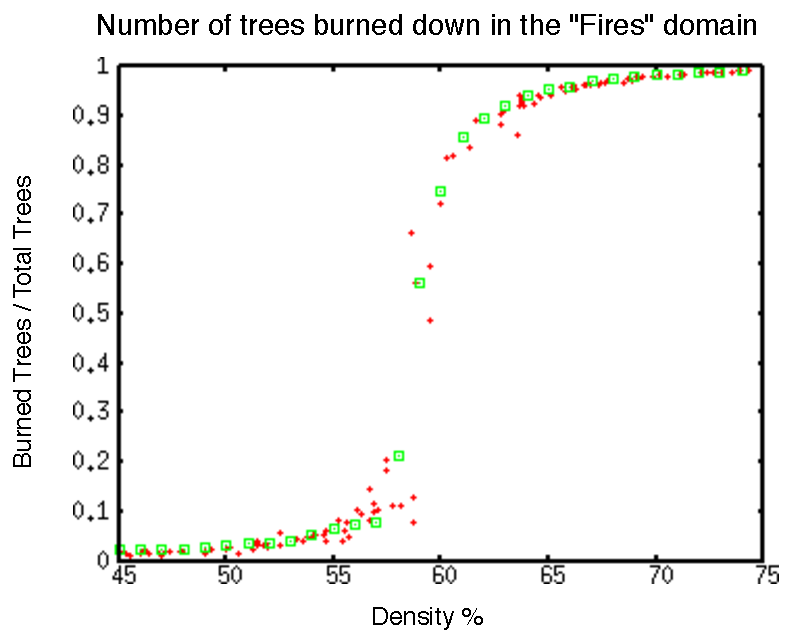
\includegraphics[scale=.5]{images/rii2.pdf}
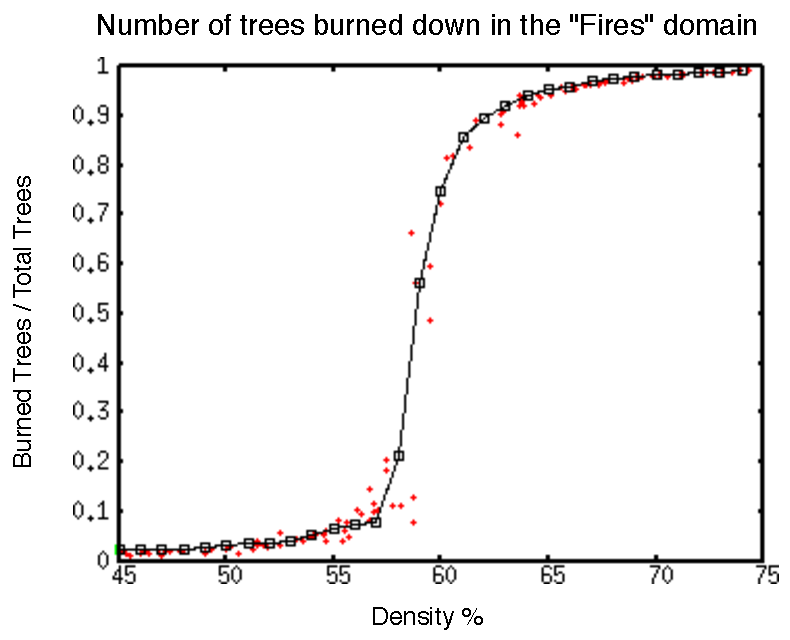
\includegraphics[scale=.5]{images/rii3.pdf}
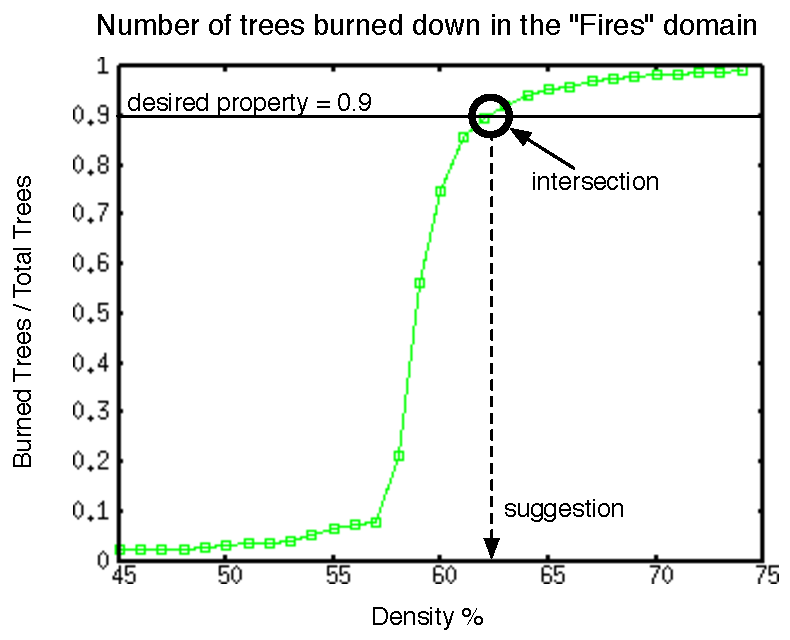
\includegraphics[scale=.5]{images/rii5.pdf}
\caption{The progression of SCI in the Fires ABM from raw data set (top left), to intersection (bottom right). }
\label{fig:rii}
\end{figure}

Next, SCI finds the intersection between the behavior space and a desired system-level property behavior $b = Burned~{ }Trees / Total~{ }Trees = 0.9$ (see bottom right image in Figure \ref{fig:rii}).
This is done by checking each simplex to see if $0.9$ is within the range of the minimum value and maximum value for $b$ in each simplex.
The only segment that intersects the $0.9$ plane is the one between 63\% and 64\%.
The intersection between this segment and the line is calculated, which in this case is approximately at $Density = 63.1$\%.

Therefore, setting $Density = 63.1$\% will be expected to yield 90\% of the trees burned down.
In higher dimensional domains, the number of points that will satisfy the system-level property will be infinite instead of just one point, since they lie on a continuous hyperplane.





\subsection{Alternative: Optimization}

\subsection{Alternative: Functional Inversion}
\label{subsec:funcinvert}

\subsection{Special Case: Classification}

\subsection{Special Case: One-to-One Mapping}

\section{Using Reverse Mappings}





\section{Evaluation Criteria}

\subsection{Time Required for Preprocessing}

\subsection{Time Required for Querying}

\subsection{Accuracy of the Reverse Mapping}


\section{Summary}




